% This template was initially provided by Dulip Withanage.
% Modifications for the database systems research group
% were made by Conny Junghans,  Jannik Strtgen and Michael Gertz

\documentclass[
     12pt,         % font size
     a4paper,      % paper format
     BCOR=10mm,version=first,     % binding correction
     DIV=14,version=first,        % stripe size for margin calculation
%     liststotoc,   % table listing in toc
%     bibtotoc,     % bibliography in toc
%     idxtotoc,     % index in toc
%     parskip       % paragraph skip instad of paragraph indent
     ]{scrreprt}

%%%%%%%%%%%%%%%%%%%%%%%%%%%%%%%%%%%%%%%%%%%%%%%%%%%%%%%%%%%%

% PACKAGES:

% Use German :
\usepackage[english]{babel}
% Input and font encoding
\usepackage[latin1]{inputenc}
\usepackage[T1]{fontenc}
% Index-generation
\usepackage{makeidx}
% Einbinden von URLs:
\usepackage{url}
% Special \LaTex symbols (e.g. \BibTeX):
%\usepackage{doc}
% Include Graphic-files:
\usepackage{graphicx}
% Include doc++ generated tex-files:
%\usepackage{docxx}
% Include PDF links
%\usepackage[pdftex, bookmarks=true]{hyperref}
\usepackage{csquotes}

% Fuer anderthalbzeiligen Textsatz
\usepackage{setspace}

% hyperrefs in the documents
\usepackage[bookmarks=true,colorlinks,pdfpagelabels,pdfstartview = FitH,bookmarksopen = true,bookmarksnumbered = true,linkcolor = black,plainpages = false,hypertexnames = false,citecolor = black,urlcolor=black]{hyperref} 
%\usepackage{hyperref}


%%%%%%%%%%%%%%%%%%%%%%%%%%%%%%%%%%%%%%%%%%%%%%%%%%%%%%%%%%%%

% OTHER SETTINGS:

% Pagestyle:
\pagestyle{headings}

% Choose language
\newcommand{\setlang}[1]{\selectlanguage{#1}\nonfrenchspacing}

\usepackage{biblatex}
\addbibresource{references.bib}

\begin{document}

% TITLE:
\pagenumbering{roman}
\begin{titlepage}
     \vspace*{1cm}
     \begin{center}
          \vspace*{3cm}
          \textbf
          {
               \Large University of Heidelberg\\
               \smallskip
               \Large Institute for Computer Science\\
               \smallskip
               \Large Working group database systems\\
               \smallskip
          }

          \vspace{3cm}

          \textbf{\large Bachelor thesis}

          \vspace{0.5\baselineskip}
          {
               \huge
               \textbf{Messaging Architecture for Integration of Customer Self-Services}
          }

     \end{center}

     \vfill
     {
          \large
          \begin{tabular}[l]{ll}
               Name:                 & Jonas Gann              \\
               Matriculation number: & 3367576                 \\
               Supervisor:           & Prof. Dr. Michael Gertz \\
               Date of submission:   & \today
          \end{tabular}
     }

\end{titlepage}

\onehalfspacing

\thispagestyle{empty}

\vspace*{100pt}
\noindent
I assure that I have written this bachelor thesis on my own and only used the specified sources and resources and that I followed the principles and recommendations "Responsibility in Science" of the University of Heidelberg.

\vspace*{50pt}
\noindent

\underline{\phantom{mmmmmmmmmmmmmmmmmmmm}}

\medskip
\noindent
Date of Submission: \today
\newpage

\chapter*{Zusammenfassung}

\newpage

\chapter*{Abstract}

\newpage

\tableofcontents
\cleardoublepage
\pagenumbering{arabic}

\chapter{Context}
Since invention of the World Wide Web, the number of its users increased rapidly. Today, more than 90 percent of the German population use the Internet \cite{Onlinestudie}. Enterprises and organizations recognised this potential to inform and interact with a large number of people. A frequently used method is "online self-service" (OSS). Specialized software tools enable customers to use services through the internet without direct human interaction.

Developing and maintaining these tools and the underlying architecture can be a difficult and expensive task. Required software solutions can therefore be accessed from commercial OSS providers. In order to use their tools, enterprises will have to integrate them into existing system architectures. Depending on for example the complexity of the tools, different integration approaches can be applied.

Many tools require user profiles if authentication, communication or access to personal information is necessary. Systems providing profiles therefore are part of numerous enterprise architectures. This leads online customers to create multiple user profiles - one for each enterprise. It is then his responsibility to keep his profiles synchronised and up to date. Increasing numbers of user profiles lead to a variety issues: Frequent changes of credentials become unrealistic and modification of an E-Mail address becomes a major inconvenience.

An evolutionary step in customer profile management is the usage of self-sovereign identities (SSI): instead of each enterprise, the customer provides a user profile. This profile can be managed by a trusted OSS provider for SSI.

In order for this concept to work, each enterprise will have to integrate the provider into their existing user profile systems. The result would be one user profile for one person which identifies him as a customer for multiple integrated enterprises.

A currently relevant example for usage of OSS with particular interesting requirements for user profiles is the "Online Access Law" (OZG). It requires all administrative services of the German federal republic, each member state and commune to be digitally available through interoperable user profiles. The current plan is to make the profile only available for usage in context of the OZG. From a user perspective, this would be yet another profile to manage.

\chapter{Objective}
Based on the prominent example of the OZG, the bachelor thesis will construct a message based integration architecture which enables system architectures with existing user profiles to accept SSI through its providers.
The goal of the integration architecture in the example is to make important OZG scenarios accessible with usage of self-sovereign identities instead of the existing user profiles.
The two points of integration are on one hand-side the system architecture relevant for the OZG in form of a list of system components and on the other hand-side the SSI provider in form of a connector.
Integration patterns are used to formulate the integration architecture which enables to use a combination of established and tested messaging solutions. In order to save investments the integration reuses as many system components as possible and modifies as few system components as necessary.

\chapter{Structure of Work}

In the beginning, the terms OSS, OSS provider, SSI, SSI provider, SSI connector and OZG are defined and the underlying concept is explained.

Then, preparatory work relevant for the integration architecture is presented. Based on process diagrams of digitalized administration services, several use cases of OSS are listed and evaluated for their relevance. They provide important information on which functionalities the SSI provider is expected to have and the integration architecture is required to integrate.

An integration approach through a connector is used. Concrete functionalities and interfaces of a possible connector are specified for usage by the integration architecture.

Based on documentation of system architectures of several member states, relevant components of the architecture relevant for the OZG are selected. Each component is explained in detail along with the functionalities it provides for usage by the integration architecture.

The integration architecture integrates previously documented connector and components of the system architecture in order to make the selected use cases available through the SSI provider. The architecture is presented iteratively. Each iteration contains increasingly demanding requirements along with the documentation of the increasingly complex integration architecture. Each documentation is done through textual explanations, multiple flow diagrams and one messaging architecture.

In order to validate the integration architecture, the execution of one administration service through the SSI provider is evaluated in theory.

\chapter{Fundamentals}
The goal of this chapter is to define terminology and to explain basic concepts for better understanding of context and objective of the bachelor thesis.


\section{Online Self-Service}
Self-service has existed for a long time. It generally means the consumption of some service without human interaction but rather in a self-reliant way. One example which is still relevant today are restaurants offering buffets. Instead of a waiter, customers take food for themselves - in self-service. In spring, some farmers allow people to pick flowers from the acre in exchange for a small fee.

In recent decades technology made advanced methods of digital self-service possible. Money can be withdrawn from local ATMs and train tickets can be bought from ticket machines. Technological advancements, at least directed to the average consumer, can be seen as advancements in self-service capabilities. Consumers buy technology which makes them independent from the help of other people. 

Since the internet enabled the connection of a very large amount of people, especially the world wide web made it accessible to the general public. The world wide web enables any user to access and interact with technological systems all over the world through a user friendly visual interface. Today, many of those systems are provided by enterprises and other organizations for customers and users to access their services - they enable customers online self-service (OSS).

Online self-service is defined as: self-reliant consumption of services over the internet without human to human interaction.

Depending on the reasoning most websites on the WWW can be described as providing online self-service. OSS therefore rather describes a perspective on the WWW than a use case.

Tow categories of OSS can be differentiated: The information category contains cases where users are enabled to retrieve relevant information. The transaction category contains cases where users modify the systems they interacts with to for example save data or trigger some internal business process.

An example for retrieving information through OSS are so called "WiKi" pages. Similar to the famous website "Wikipedia", information about for example the usage of a product can be made accessible to customers. In this case, it is not necessary any more to call a support hot-line.
Another example are online learning platforms which provide customers with necessary information to for example learn a language. In this case, it is not necessary any more to meet teachers.
Online job hunting websites enable its users to find information about job offers which fit their requirements. In this case it is not necessary any more to visit employment bureaus.

A common use case for transaction through OSS are online retailers which enable users to start payment and delivery processes. They are often accompanied by OSS for information in order to find and select products. In this case it is not necessary any more to go to the local shopping mall.
Another use case is the management of user identities which enables users to authenticate themselves and manage personal information. In this case it is not necessary any more to show up in person at for example a store in order to identify ones identity and give personal information about for example the living address.

Reasons for the widespread usage of online self-service are significant benefits in ease of service usability for customers and cost reduction for enterprises. Customers can self-service from almost every place, easily manage customer data like phone number and address, configure services like subscription plans and access lots of information on available products or trouble shooting steps in an immediate way. Online customer self-service improves usability, saves time, increases availability, saves money and therefore increases customer experience. Enterprises, especially in progressive countries, aim to keep employment at a minimum, as it is a big cost factor.

Digital self-service turns customers into unpaid employees.

\subsection{OSS Provider}
In order for customers to use online self-service, companies and institutions have to provide the necessary software tools. Depending on category and use case of OSS, different software tools exist.

A chain of stores might provide tools which enables the users to inform themselves about available products and opening hours. This could for example be a search functionality for stores in the local area and a catalogue of available products of a selected store. Online retailers however will require additional tools which for example enable management of user profiles to authenticate and communicate with customers.

OSS providers are defined as: enterprises which develop and maintain solutions for OSS and make them accessible to system architectures of customers. 

Depending on the complexity of the solution, different methods of access are possible. One possibility would be to provide a self-contained software, the customer can deploy in his system architecture. This can be done for example in the case of solutions for WiKi-pages where the customer installs respective software in his web server. Another possibility would be, for the OSS provider to host the solution himself and provide system architectures of customers access. This can be done for example in the case of retailers which contain systems only for managing a catalogue of available products and processing incoming orders. They could integrate an online shop solution hosted by a OSS provider through using a business connector.

\section{SSI}

\section{SSI Connector}

\section{OZG}

This section introduces the law for improvement of online access of administrative services (Online Access Law - OZG), its origin, purpose and planned realization.

\subsection{Context}

The Federal Ministry of the Interior, Building and Community is, amongst other things, responsible for modernizing public administration \cite{BMI:Moderne_Verwaltung}. Current modernization efforts lie in the construction of an E-Government \cite{BMI:Behoerdengaenge}.
The E-Government-Law in 2013 was an early step increasing internal usage of digital systems in governmental administration. This includes for example the usage of digital personal files and scanning of documents for replacement \cite{BMI:E-Government_Gesetz}. 
In 2017 the German government passed the law for improvement of online access to administrative services (OZG) which focuses on usage of administration services by the people \cite{BMI:Onlinezugangsgesetz}. 
Modernization of the administration, however, is not exclusive to Germany as in 2018 the European Parliament and Council decided on a Single Digital Gateway (SDG) providing uniform access to digital administrative governmental services of every European country \cite{BMI:Single_Digital_Gateway}.

\subsection{Motivation}

Customers on the free market are used to One-Stop-Shops providing access to services of companies in one digital place. Many self-service methods improve the user experience: Customers of e-commerce companies can put products in a digital shopping card, pay with digital money and select a location for delivery. In most cases, no direct human to human interaction is required. Customers complete the process of ordering in self-service. The progress of online self-service usage on the free market is a result of the ongoing digitalization of the world and the competitiveness of the market. Today, many customers own personal computers or smartphones and companies providing easy access to their services via online self-service have an advantage in the market.
Governmental institutions provide administrative services for customers. This can for example be an application for child benefit or a new ID card. In contrast to the free market, access to administrative services is, in most cases, not available through online self-service. Reasons are, that digitalization is expensive and governmental institutions do not have competitors.
Digitalization of governmental administration could for example enable users to inform themselves about available administrative services and access them over the internet. The need to personally appear in offices of an administration would be reduced. Communication about questions or required documents could also happen faster, more immediate, and more reliable over the internet than over mail. Governmental institutions could reduce bureaucracy through modernization of registries and the once-only principle.
The German government recognizes the possible improvements and presents, amongst other things, the OZG as a solution. \cite{IT-Planungsrat:Herausforderung}

\subsection{The OZG}

The law for improvement of online access of administrative services (Online Access Law - OZG) passed in 2017 and requires federal republic and member states to execute the following regulations until 2022 \cite{BMI:OZG_Wortlaut}:
\begin{enumerate}
    \item \textbf{Digital availability of administrative services} \\
    An administrative service is the electronic processing of administrative procedures which are available from outside the governmental institution.  As it is not clear which administrative services exactly are meant by the definition of the OZG, the BMI created a catalogue \cite{BMI:Verwaltungsleistungen}. The OZG requires these services to be digitally available. As a guideline to what is considered sufficient availability, the BMI defined a maturity model \cite{BMI:Digitale_Services}.
    \item \textbf{Digital access to administrative services through administration portals of a portal network} \\
    Federal republic, each member state and each commune must provide an administration portal. Portals of communes must be linked to the portal of the corresponding member state. Portals of federal republic and member states must be connected through a portal network. \cite{BMI:Portalverbund} Each portal must provide a "seek and find" feature, which enables users to find all administrative services provided by any administration portal \cite{Cotar:Drucksache_19/19089}. 
    \item \textbf{Interoperable user profiles for accessing administrative services} \\
    Federal republic and member states must provide user profiles which can be used to identify the corresponding person while requesting access to administrative services, to save personal information according to the once-only principle, to receive and send messages via a digital mailbox and to pay for services \cite{Cotar:Drucksache_19/19089}. The user profiles must be interoperable for every administration portal of the portal network.
\end{enumerate}

\subsection{OZG Execution}

Execution of the OZG can be separated into two projects: Digitalization and Networking. Digitalization focuses on transformation of existing processes and services to be using modern technologies. This includes most importantly the digitalization of governmental administrative services. The networking focuses on connecting existing and future governmental systems to make digitalization universally usable. This includes most importantly the construction of administration portals which are connected in a portal network.

Many services, which are still bound to paper must be digitalized. In total, the BMI lists 575 relevant services. Some of them are provided by the federal republic, some by the member states and yet other by the communes. Respective to these responsibilities, the task of digitalization is distributed between federal republic and member states, where each member state is assigned to take the lead for specific areas. \cite{BMI:Onlinezugangsgesetz} Results of the digitalization are documented on the "OZG-Informationsplattform" \cite{BMI:Informatiosplattform} as process diagrams and data schemata.

Administrative services are made available through administrative portals which are be provided by federal republic, each member state and each commune. Communes integrate their portals with corresponding member states. The portals are connected through an "Online-Gateway" and form a portal network.

Federal republic and each member state provide digital access to administrative services. An important method is called "one for all": One member state manages the digitalization of a category of administrative services and makes them digitally accessible for every other member state. Every administrative service can be found through a search function provided by every portal of the network.

Depending on the administrative service, a user profile is required to verify ones identity. As federal republic and most member states already provide their own user profiles, the "IT-Planungsrat" decided to save investments by connecting them to an interoperable user profile.

There exists a low, substantial and high level of authentication security when logging in to a user profile or when creating one.
A low trust level is for example the usage of a username and password combination, a high trust level is for example the usage of the eID feature of the German ID card. Depending on the administrative service a profile tries to access, a different trust level is required.

Profiles also enable users to save personal data in a data wallet and to communicate with institutions through an inbox.

\chapter{Preparatory Work}

\section{OZG OSS Scenarios}

The information platform of the OZG contains information about many administration services in form of process diagrams \cite{BMI:Ergebnisse}. They serve as a resource to identify important OSS scenarios of administration processes. The following scenarios were identified:

\subsection{Identity Management}

\subsubsection{Scenario Profile Management}
\begin{itemize}
    \item Create a user profile
    \item Delete a user profile
    \item Check existence of a user profile
\end{itemize}

\subsubsection{Scenario Identity verification}
\begin{itemize}
    \item Login to a user profile
    \item Provide multiple levels of security for identity verification
    \item Usage of a guest profile
\end{itemize}

\subsection{Request Management}

\subsubsection{Scenario Request Preparation}
\begin{itemize}
    \item Search for administration services
    \item Check necessity of a profile
    \item Check required level of identity verification
    \item Selection of institution responsible for processing the request (Specification of current location)
\end{itemize}

\subsubsection{Scenario Request Creation}
\begin{itemize}
    \item Filling in a form for an application
    \item Automated filling in of form with saved personal data
    \item Collaboration on application by multiple identities
\end{itemize}

\subsubsection{Scenario Request Delivery}
\begin{itemize}
    \item Transmission of an application to responsible institution
\end{itemize}

\subsubsection{Scenario Request Processing}
\begin{itemize}
    \item Period of validity of applications
    \item Notification of user about missing information or documents
    \item Transmission of missing information
    \item Notification of user about required preliminary administration services
    \item Communication through E-Mail
    \item Cancel an application
    \item Approvals of user to e.g. data protection or information transfer
    \item Modification request of application after transmission
    \item Notification of received application by institution
    \item Request status update by user
    \item Sending notification to confirm the reading of a message
    \item Notification of certain events to separate person e.g. parents
    \item Request of institution about explicit document
\end{itemize}

\subsubsection{Scenario Request Finalization}
\begin{itemize}
    \item Notification of outcome of process / application
    \item Objection of user to result of the process
    \item Access to signed digital formula of result of process
    \item Definition of dates for evens
\end{itemize}

\subsection{Data Management}

\subsubsection{Scenario Access Management}
\begin{itemize}
    \item Access to an application by multiple separate identities
    \item Sharing of documents saved in a wallet
\end{itemize}

\subsubsection{Scenario Data Consistency}
\begin{itemize}
    \item Period of validity of documents
    \item Profile data discrepancies between involved user profiles
\end{itemize}

\subsubsection{Scenario Data Accessibility}
\begin{itemize}
    \item Upload of e.g. documents and certificates
    \item Saving personal data entered in a form to the user profile
    \item Protocol of all processes accessible with information about interactions
\end{itemize}

\section{OSS Connector}

\section{OZG System Architecture}
This section describes the system architecture of a member state relevant for the execution of the OZG an integration of a OSS provider. Due to a lack of detailed information, the system architecture is described by components responsible for a category of tasks. Each component is associated to data objects it processes. The definition of components and data objects are based on research about planned system architectures of member states.

\subsection{User Profile}
Each member state provides its own user profile which manages the identity of a user. It enables him to create, delete and login to a profile, authenticate for administration services, communicate with institutions through an inbox and manage personal information and documents in a data wallet.

\subsection{Administration Portal}
The administration portal provides the user with a web-interface he can use to access his user profile and search for available administration services.

\subsection{Application Platform}
The application platform gives access to administration services by providing the user with a website he can use to fill in application forms and sent them to the responsible institutions. It is possible to prefill the form with personal data stored inside the user profile.

\subsection{Institution}
Institutions are the entities distributed all over the member state which eventually process the incoming applications and provide the users with solutions.

\chapter{Integration Architecture}

This chapter presents a message based integration architecture which enables access to OSS features of member states through a OSS provider. Multiple versions of an integration architecture are presented which fulfill increasingly complex requirements. Requirements are formulated as user scenarios which should be accomplishable through the OSS provider.
Each version is presented in the form of multiple flow charts, each describing sequential steps while carrying out a required scenario and a corresponding messaging infrastructure.

\section{Basic}

\subsection{Requirements}
In the first version of the integration architecture, users of the OSS provider should be able to
\begin{itemize}
    \item fill in an application
    \item authenticate
    \item receive and send messages
\end{itemize}

\subsection{Flow Charts}

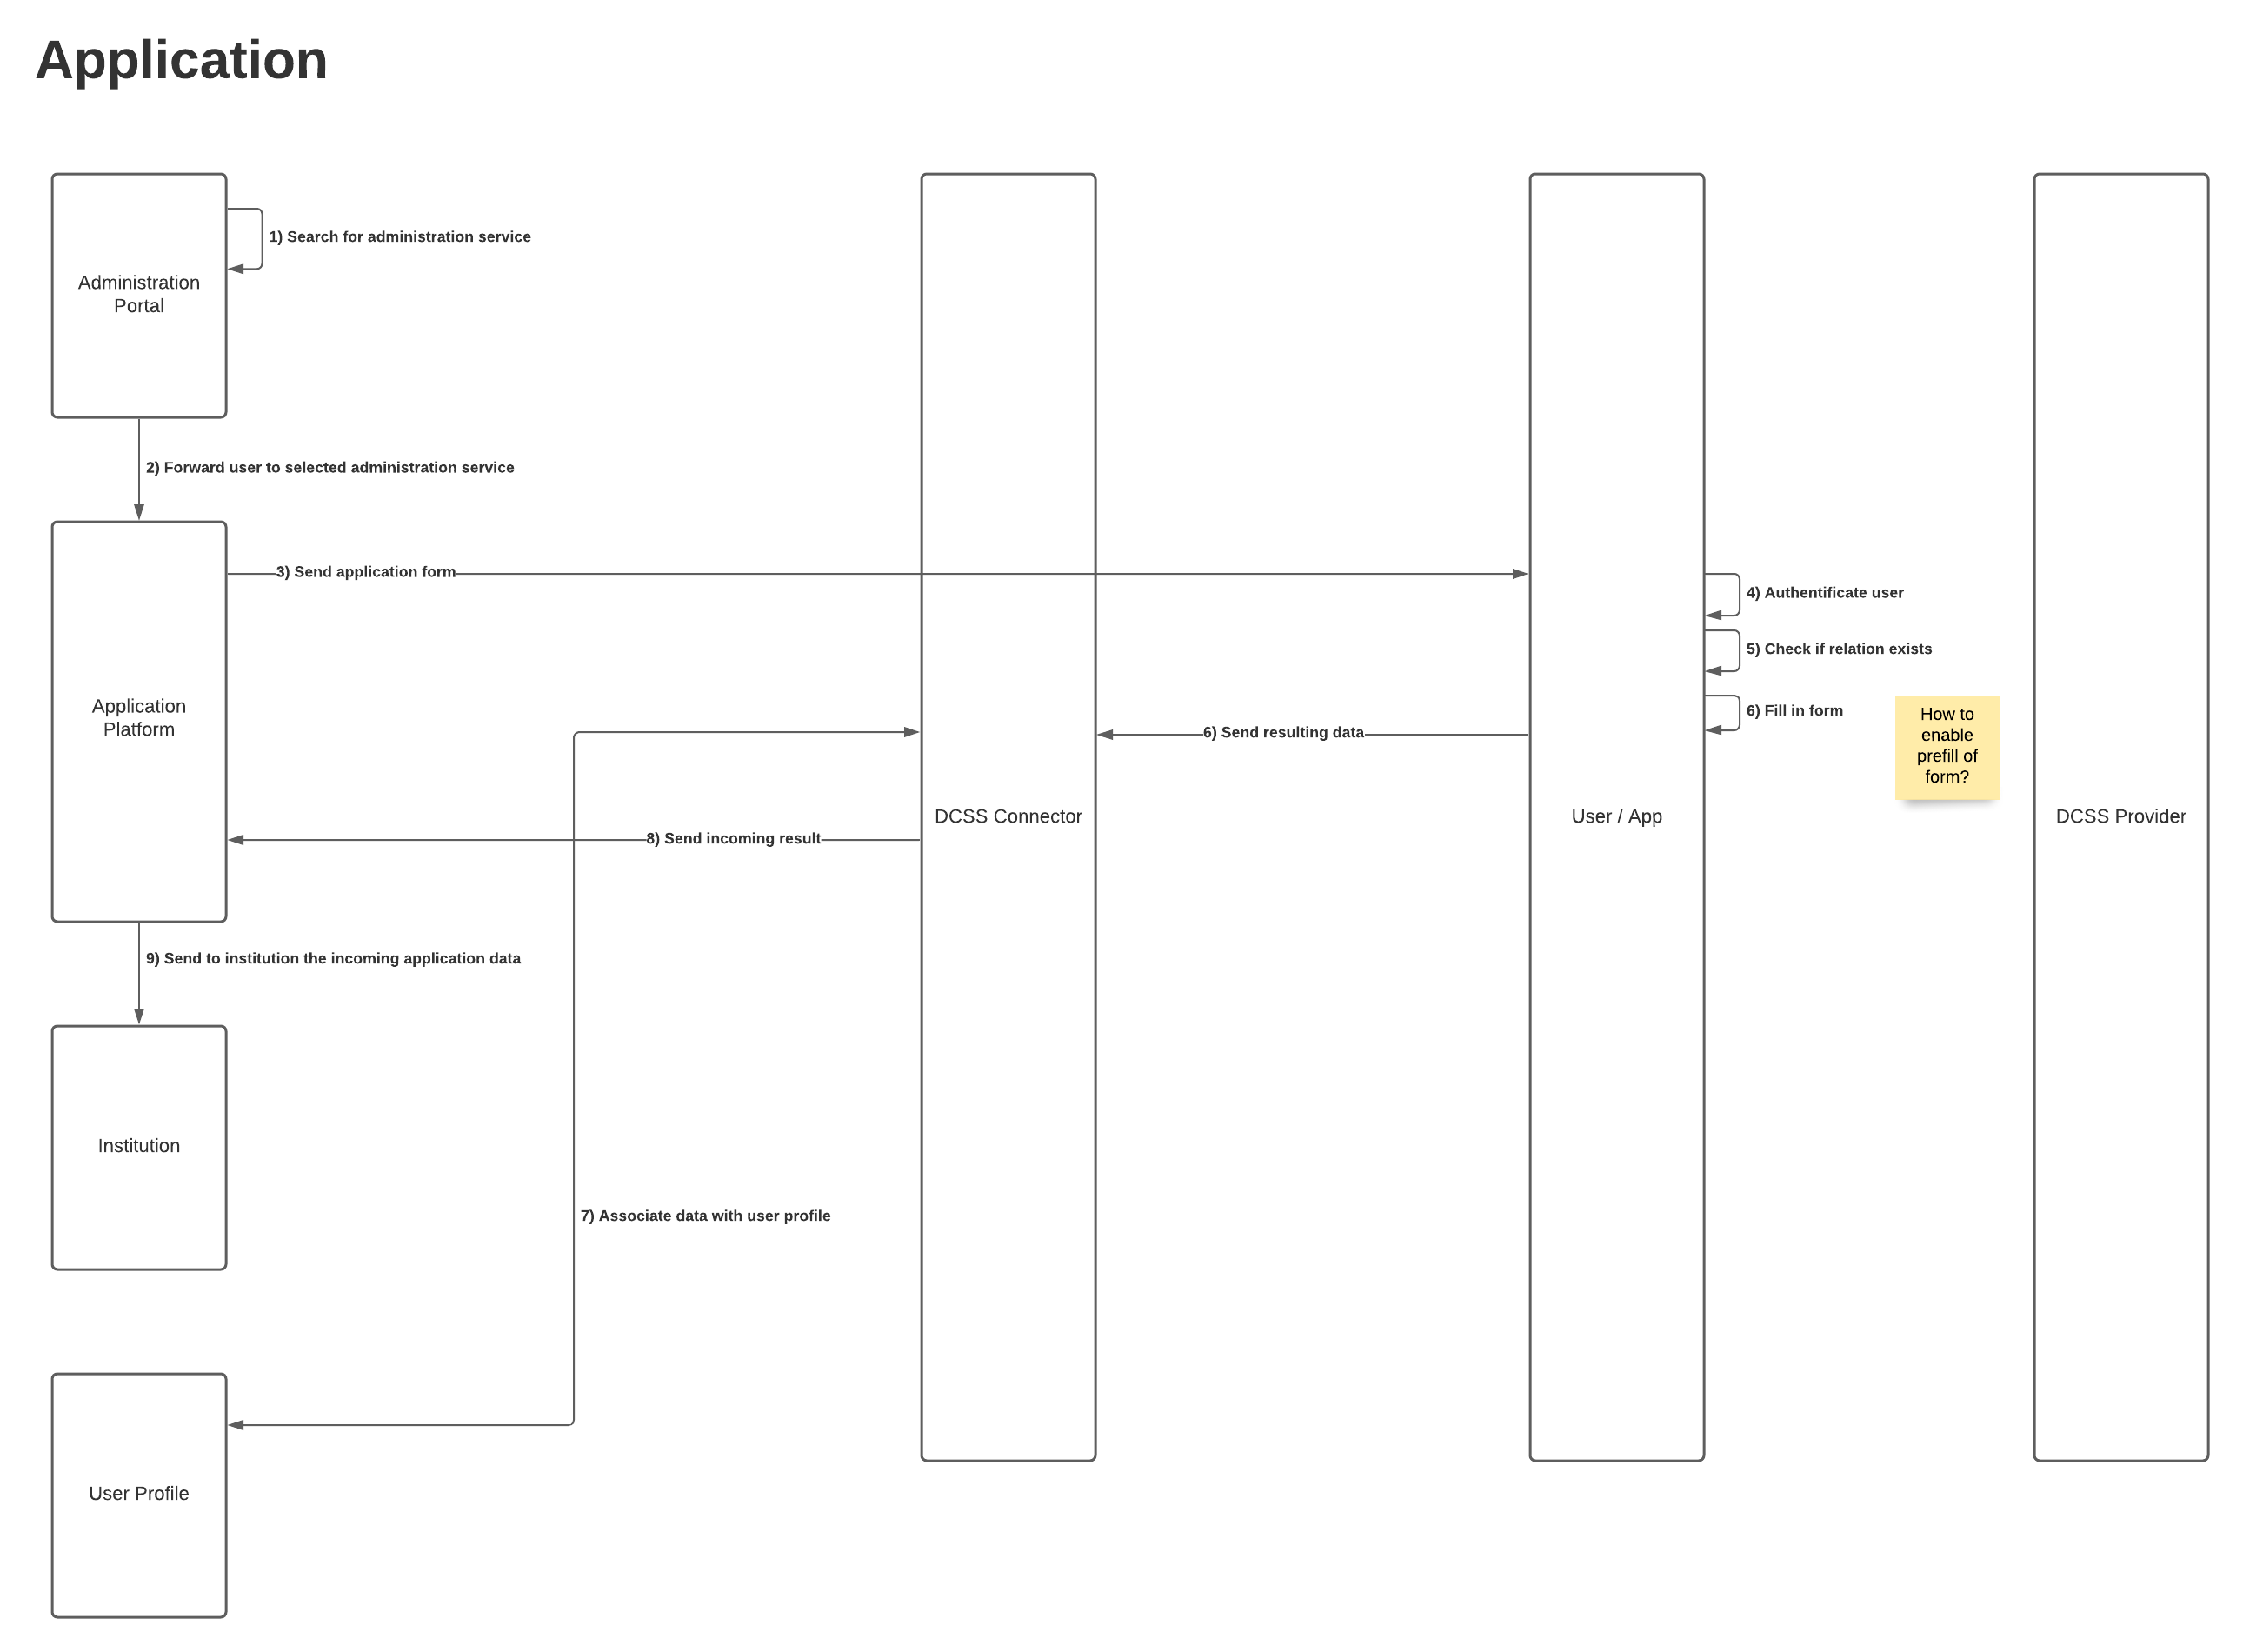
\includegraphics[width=\textwidth]{Basic Integration Application.png}

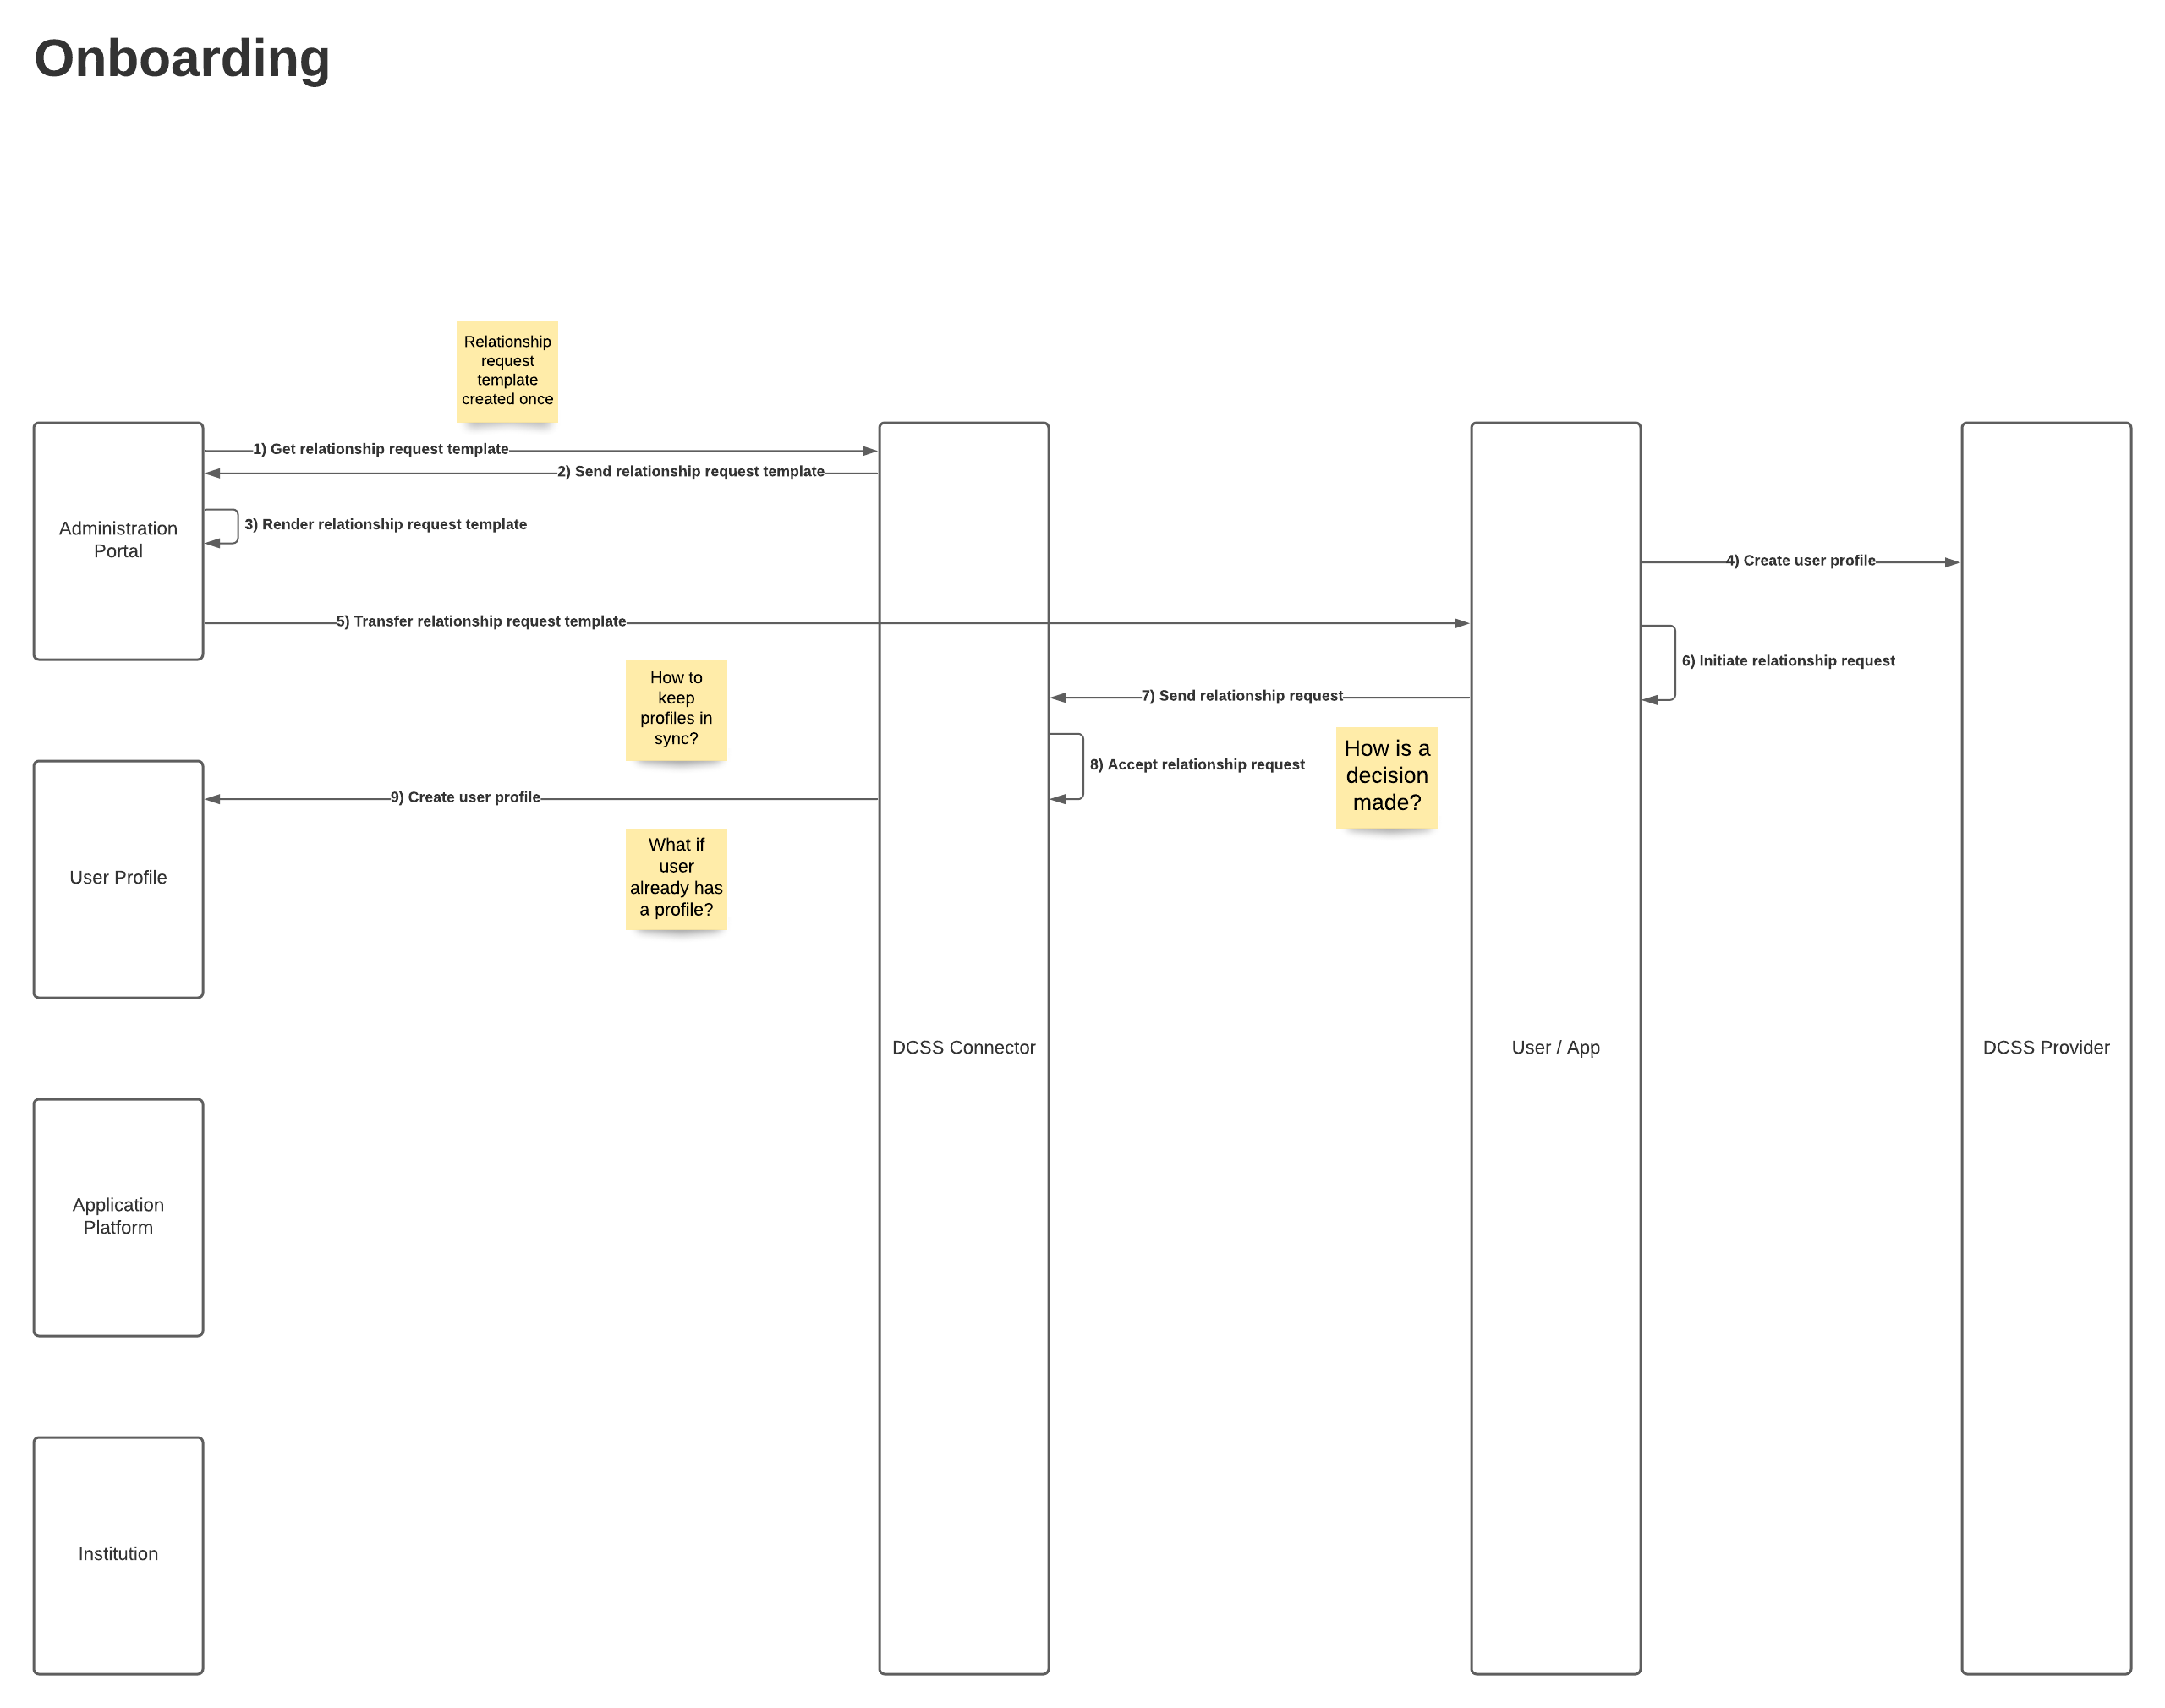
\includegraphics[width=\textwidth]{Basic Integration Onboarding.png}

\subsection{Messaging Integration}

\section{Advanced}

\subsection{Requirements}

\subsection{Flow Charts}

\subsection{Messaging Integration}


\chapter{Integration Architecture Evaluation}

\section{Technology}

\section{Customer Example}

\section{Operating Manual}

\chapter{Outlook}

\begin{itemize}
     \item Expanding integration architecture with capabilities for OSS scenarios of different areas than online administration self-service
     \begin{itemize}
          \item online payment self-service (PayPal, psd2)
          \item online shopping self-service (Amazon)
          \item online health care self-service (DVG)
          \item online entertainment self-service (Netflix, YouTube, Spotify)
          \item online information / support self-service (StackOverflow)
     \end{itemize}
\end{itemize}

\printbibliography


\end{document}
